\newpage
\visHeader

\begin{figure}[htbp]
  \centering
  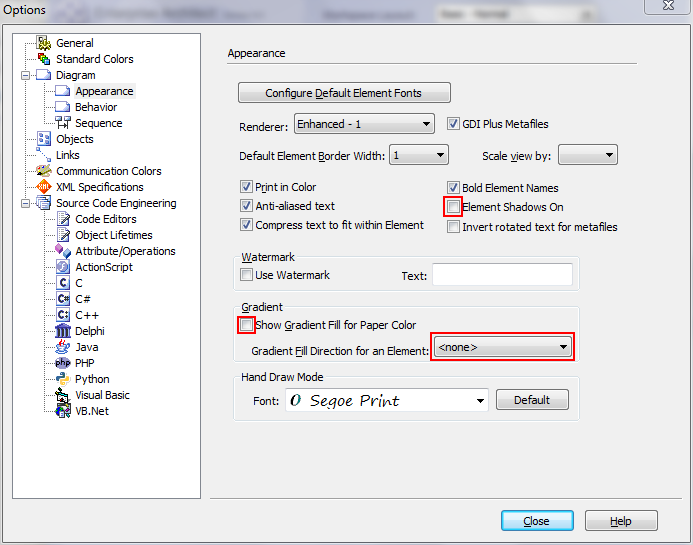
\includegraphics[width=0.8\textwidth]{standardAppearance}
  \caption{Our choice of the standard appearance for model elements.}
  \label{fig_standardAppearanceEA}
\end{figure}

in EA lingo, and is used as a  container to group a set of related \emph{packages}. 
In our case, \texttt{Demo}  consists of a single package \texttt{DoubleLinkedListLanguage}.
An EA project however, can consist of numerous models that in turn, group numerous packages.


% Must change to 'projects first' here?
Now switch to your \emph{Eclipse workspace} and note the two nodes named \texttt{Spe\-ci\-fi\-ca\-tions} and \texttt{Demo}.  These nodes, used to group related \emph{Eclipse projects} in an Eclipse workspace, are called \emph{working sets}.
The working set \texttt{Spe\-ci\-fi\-ca\-tions} contains all \emph{metamodel projects} in a  workspace. A metamodel project contains a single EAP (EA project) file and is used to communicate with EA and initiate code generation by simply pressing F5 or choosing ``refresh'' from the context menu.
In our case, \texttt{Specifications} should contain a single metamodel project \texttt{Demo} containing our EA project file  \texttt{Demo.eap}.
% \% end common
 
Figure~\ref{fig_fromEAtoEclipse} depicts how the Eclipse working set \texttt{Demo} and its contents were generated from the EA model \texttt{Demo}.
Every model in EA is mapped to a working set in Eclipse with the same name. 
From every package in the EA model, an Eclipse project is generated, also with the same name. These projects, however, are of a different \emph{nature} than for example metamodel projects or normal Java projects, and are called \emph{repository projects}.  
A nature is Eclipse lingo for ``project type'' and is visually indicated by a corresponding nature icon on the project folder.
Our  metamodel projects sport a spanking little class diagram symbol. 
Repository projects are generated automatically  